\documentclass[12pt]{report}
\usepackage[pdftex]{graphicx}
\usepackage{url}
\usepackage{setspace}
\usepackage{makeidx}
\usepackage[utf8]{inputenc}
\usepackage{fancyhdr}
\usepackage{layout}
\usepackage{float}
\usepackage{titlesec}
\usepackage{graphicx}
\usepackage[a4paper,pdftex]{geometry}	% Use A4 paper margins
\usepackage[english,spanish]{babel}
\usepackage{xcolor} % Required for specifying custom colors
\usepackage{fix-cm} % Allows increasing the font size of specific fonts beyond LaTeX default specifications

\DeclareGraphicsExtensions{.pdf,.png,.jpg}

\setlength{\oddsidemargin}{0mm} % Adjust margins to center the colored title box
\setlength{\evensidemargin}{0mm} % Margins on even pages - only necessary if adding more content to this template

\renewcommand\thesection{\arabic{section}} %Section numbering
\renewcommand\thesubsection{\thesection.\arabic{subsection}} %Subsection numbering

\setlength{\voffset}{-1.2cm}
\setlength{\textheight}{650pt}
\setlength{\parindent}{0pt}
\renewcommand{\baselinestretch}{1.5}
\definecolor{grey}{rgb}{0.95,0.95,0.95} % Color of the box surrounding the title - these values can be changed to give the box a different color	

\pagestyle{fancy}
\fancyhf{}
\lhead{A Fireball for Your Friends}
\rhead{Game Design Document}
\rfoot{\thepage}

\newcommand{\sectionbreak}{\clearpage}


\makeindex

\begin{document}

\pagestyle{empty} % Remove page numbering on this page

%----------------------------------------------------------------------------------------
%	TITLE SECTION
%----------------------------------------------------------------------------------------

\colorbox{grey}{
	\parbox[t]{1.0\linewidth}{
		\fontsize{50pt}{30pt}\selectfont % The first argument for fontsize is the font size of the text and the second is the line spacing - you may need to play with these for your particular title
		\vspace*{0.7cm} % Space between the start of the title and the top of the grey box
		
		A Fireball \\ 
		for Your Friends \\ 
        \fontsize{30pt}{34pt}\selectfont
        Game Design Document		
		\par
		
		\vspace*{0.4cm} % Space between the end of the title and the bottom of the grey box
	}
}

\vspace*{0.4cm} 
{\large Un \textbf{juego de duelos mágicos multijugador en 3ª persona}}

\begin{spacing}{0.6}
Target: \textit{chicos entre 16-22 años, amantes de los juegos competitivos, mid-core} 

Plataforma: \textit{XBox One, Windows PC}
\end{spacing}


\begin{figure}[h]
    \centering
    
\includegraphics[width=0.6\textwidth]{fireball}
\end{figure}

\vfill % Space between the title box and author information

{\centering \hfill \copyright 2018 Pedro Montoto García} \\

%----------------------------------------------------------------------------------------

\clearpage

\tableofcontents

\cleardoublepage

\setlength{\voffset}{0cm}
\setlength{\parindent}{1cm}
\setcounter{page}{1}

\part{Game Overview}

\section{High Level Concept}
\pagestyle{fancy}

Un juego multijugador\footnote{Este documento se incluye como anexo a un \textit{vertical slice} del juego descrito por el propio documento, que ejemplifica la experiencia de un modo de juego de combate de dos jugadores (uno de los cuales es manejado por la IA). Todas las features implementadas en dicho \textit{vertical slice} se indican como tales en sus respectivas secciones.} (pantalla partida y online) en tercera persona donde dos equipos cada uno con de 1 a 3 magos duelean en un pequeño escenario usando hechizos variados y espectaculares. Cada jugador deberá componer su biblioteca de hechizos en cada encuentro, escogiéndolos según la utilidad que tengan para contrarrestar al enemigo y sinergizar con sus aliados. 

Cada encuentro tendrá sus objetivos, i.e. aniquilación, capturar la bandera, defender un objetivo, football (à la Rocket League)..., y su duración será corta, i.e. entre 5 y 10 minutos, para asegurar que todo el mundo pueda disfrutar de al menos una partida rápida, pero que ésta sea intensa. Podemos describir este juego en términos de ``ajedrez a la velocidad de la luz''.

La experiencia de juego se centra en hacer que el jugador sienta su maestría al derrotar a enemigos usando los diferentes hechizos, evitándolos a su vez. El loop de juego principal estará en dominar los diferentes hechizos y sus sinergias via el empoderamiento del jugador.

\begin{figure}[h]
    \centering
    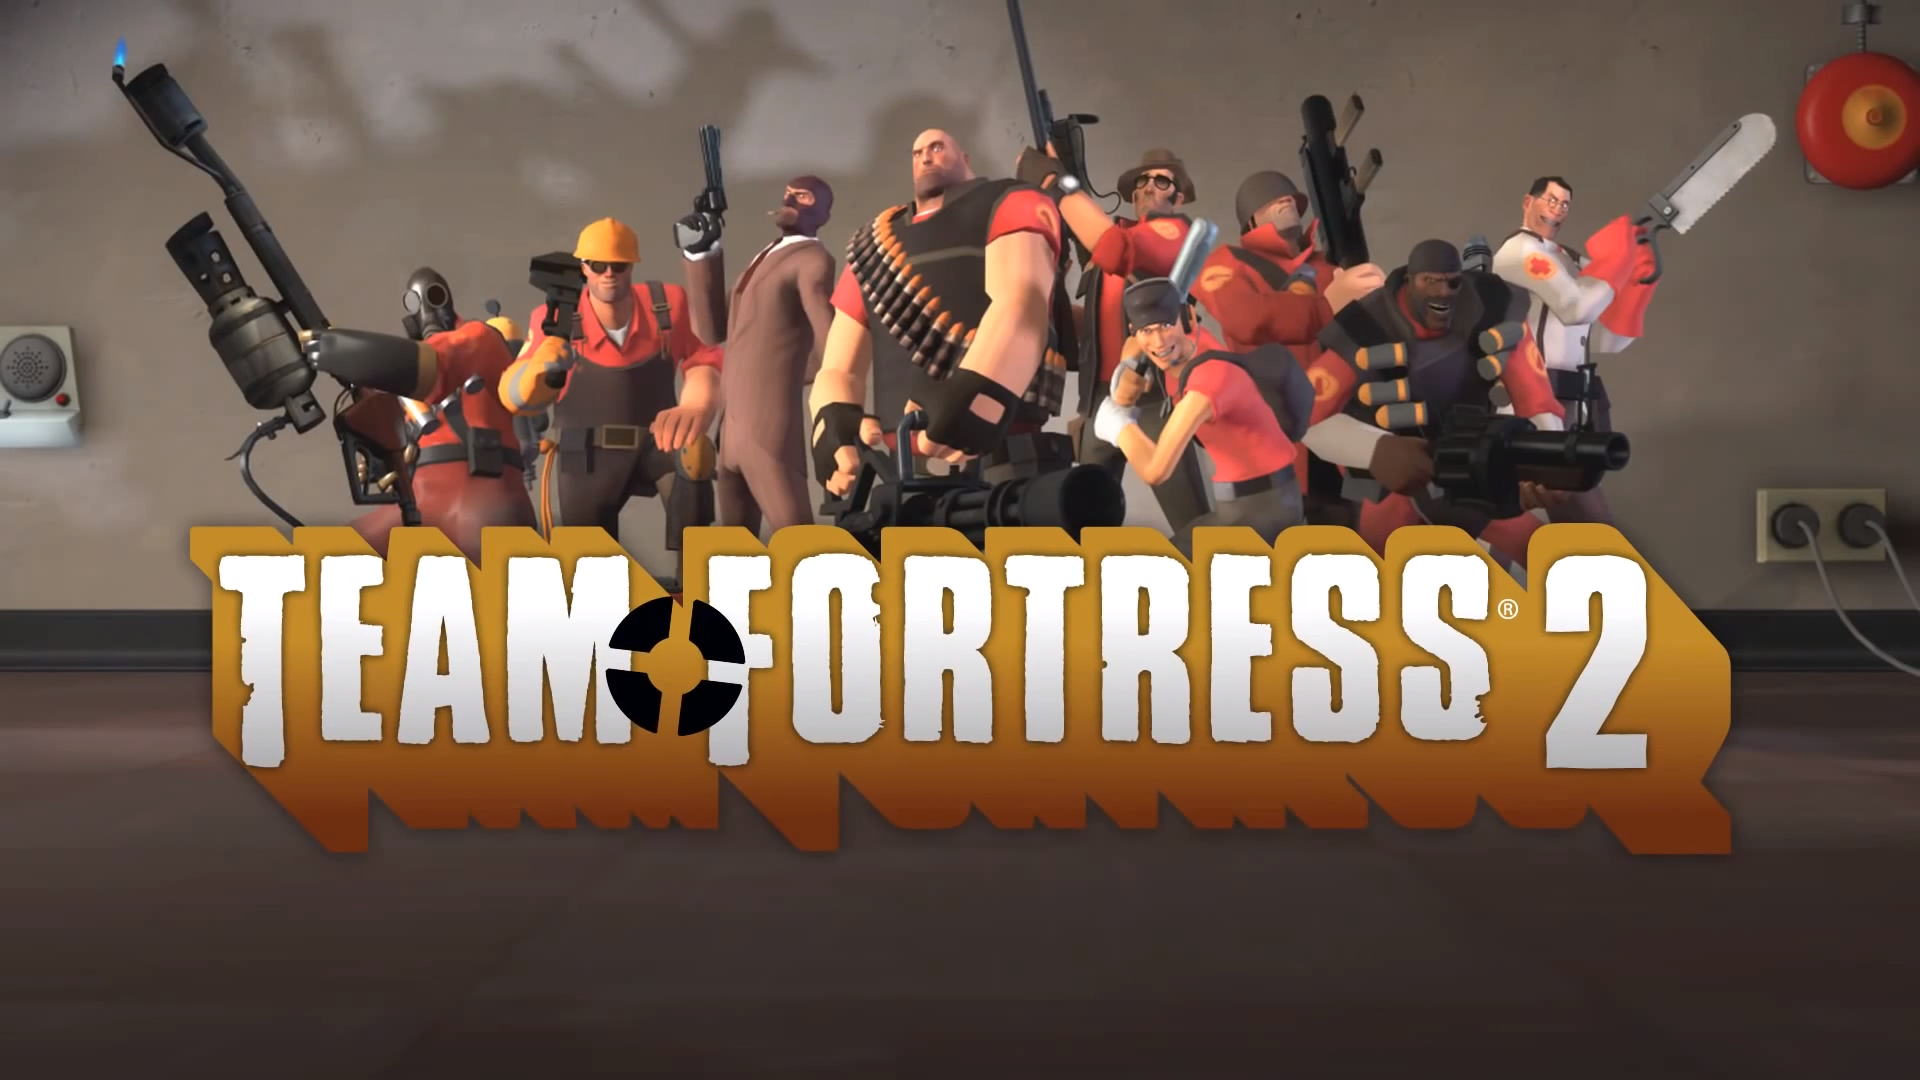
\includegraphics[width=0.8\textwidth]{tf2}
    \caption{Tomamos de Team Fortress 2 la variedad de gameplay, la velocidad de la acción y lo intuitivo que resulta para nuevos jugadores}
\end{figure}

\section{State of the Art}

\subsection{Competitors}
Este juego compite directamente con otros shooters multijugador competitivos como \textit{Call of Duty}, \textit{Battlefield}, \textit{PlayerUnknown's BattleGrounds (PUBG)} (éste en 3ª persona también), \textit{Counter Strike} etc. También entra en el mercado de los Multiplayer Online Battle Arena (MOBAs) y otros tipos de videojuego altamente competitivos, como \textit{Defense of the Ancients (DOTA)} y \textit{League of Legends (LOL)}. Dado que la temática es mágica-medieval y adulta también podría ocupar espacio de mercado de juegos de fantasía altamente centrados en gameplay en 3ª persona (con un multiplayer altamente competitivo) como la saga \textit{Dark Souls}.

\subsection{Overcoming Competitors: Unique Selling Points}
Para convencer a la gente que está jugando los juegos arriba mencionados optaremos por aprovechar:

\begin{itemize}
\item La combinación de shooter altamente competitivo con una ambientación fantástica, que no ha sido probada aún en el mercado.
\item Gameplay sólido con control altamente responsivo
\item Situaciones espectaculares que hacen fácil que el juego se promocione a sí mismo en redes sociales, mediante el reenvío de gifs o vídeos con jugadas llamativas
\item Personalización en todos los aspectos del juego (desde habilidades hasta apariencia)
\end{itemize}

\section{Visual Appeal}

\subsection{Character appeal}

Dado que no planteamos un modo historia de un sólo jugador, sino que la historia se ve símplemente como un extra que añade una capa de profundidad al modo multijugador como flavor text de hechizos y personalizaciones, en este apartado nos centraremos en conseguir una estética agradable, personal y que envejezca bien (i.e. Team Fortress, Overwatch) dado que siendo multijugador nuestro planteamiento es alargar la vida del juego lo máximo posible. Por tanto, para ello se utilizarán gráficos estilizados y simplificados adornados por gran variedad de efectos.

Otro punto importante en los gráficos es la variedad de elementos de personalización del personaje jugador, de los entornos y de los efectos de hechizo.

\subsection{Scope of Visual Effects: Visual Variety}

Estamos orientados a hacer este juego lo más espectacular y variado posible. Siendo la variedad de hechizos uno de nuestros Unique Selling Points haremos cada hechizo fácilmente reconocible por sus efectos visuales al mismo tiempo que las combinaciones que cada jugador escogerá en sus partidas sean únicas en cada una. Para conseguir ésto se utilizará todo el potencial de efectos especiales, efectos de partículas y post-procesado de pantalla completa.

\subsection{Environment Appeal}

Los entornos serán simples pero rápidamente identificables. La idea es que los entornos sirvan para aumentar la variedad de situaciones que el jugador afrontará durante sus partidas: aunque se ponga la atención en su atractivo visual éste no es el objetivo principal de nuestros entornos de juego.

\section{Gameplay Features}     

\subsection{Reward systems}

\begin{itemize}
\item Un sistema de desbloqueo de habilidades irá guiando al jugador de hechizos más simples a otros más complejos, para que su curva de aprendizaje sea menos costosa. Sistemas similares se usan en Heroes of the Storm y LOL, o el modo ``héroes simples'' en DOTA.
\item Como extensión del sistema previo, un subsistema de niveles y puntos de experiencia por partida finalizada recompensará al jugador con sistemas de personalización variados. Se establecerán quests diarias con recompensas de experiencia extras para recompensar a los jugadores que asisten al juego más regularmente.
\item Un modo de juego competitivo, desbloqueable para jugadores con experiencia por encima de lo que consideremos \textit{niveles de tutorial}, proveerá a los jugadores más hardcore de un modo de juego más acorde a sus gustos.
\end{itemize}     

\subsection{Modes of play}

El modo básico de juego es el multijugador, que permite a cada jugador conectarse a un servidor central de lobbying de partidas y jugar con sus amigos o desconocidos a través de internet. El juego también permite a jugadores juntarse en una casa, conectar la Nintendo Switch y jugar en pantalla partida compartiendo un televisor. Los jugadores pueden loguearse en sus propias cuentas y usarlas en la consola de un amigo o bien usar una copia del personaje del dueño de la consola con colores cambiados.

El juego ofrece un modo de práctica contra maniquíes de mago, para probar y practicar habilidades \footnote{En esto consiste el \textit{Vertical Slice}.}. El core del juego será la elección de ``modo de dificultad'' multijugador:

\begin{description}
\item[Quick Play:] Modo ``Casual'' de partidas rápidas
\item[Competitivo:] Modo ``Serio'' donde se asume mayor habilidad y coordinación dentro del equipo
\end{description}

En Quick Play o Competitivo pueden jugarse los siguientes modos:

\begin{description}
\item[Exterminación:] Equipos de Magos intentan matarse unos a otros con un límite de tiempo. Gana el equipo que tenga más componentes vivos al final del límite de tiempo o que consiga matar a todos los enemigos dentro de dicho límite. \textit{Implementado en el Vertical Slice}.
\item[Capturar la Bandera:] Existen bases para cada equipo y cada una guarda una bandera. El objetivo es entrar en la base enemiga y llevar la bandera enemiga a la base propia. Gana el equipo que más puntos tenga al final del límite de tiempo.
\item[Football:] El entorno de juego es un campo libre con dos ``porterías'' en los extremos, cada una de un equipo. El modo de juego consiste en combinar la lucha con el uso de los hechizos para meter la pelota en la portería contraria. Gana el equipo que más goles tenga al final del límite de tiempo.
\item[King of the Hill:] Se designa una zona especial de captura en el mapa, con un tiempo límite para cada equipo. El tiempo límite de cada equipo desciende hacia 0 mientras la zona de captura está en sus manos. Gana el primer equipo que lleve a 0 su contador de tiempo límite.
\end{description}
\part{Gameplay Description}

\section{Control}

\subsection{Controller Config}

El juego actualmente cuenta con controles para teclado y ratón, pero se recomienda jugar con un mando estilo XBox (360 / One) y la siguiente configuración.

\begin{figure}[h]
    \centering
    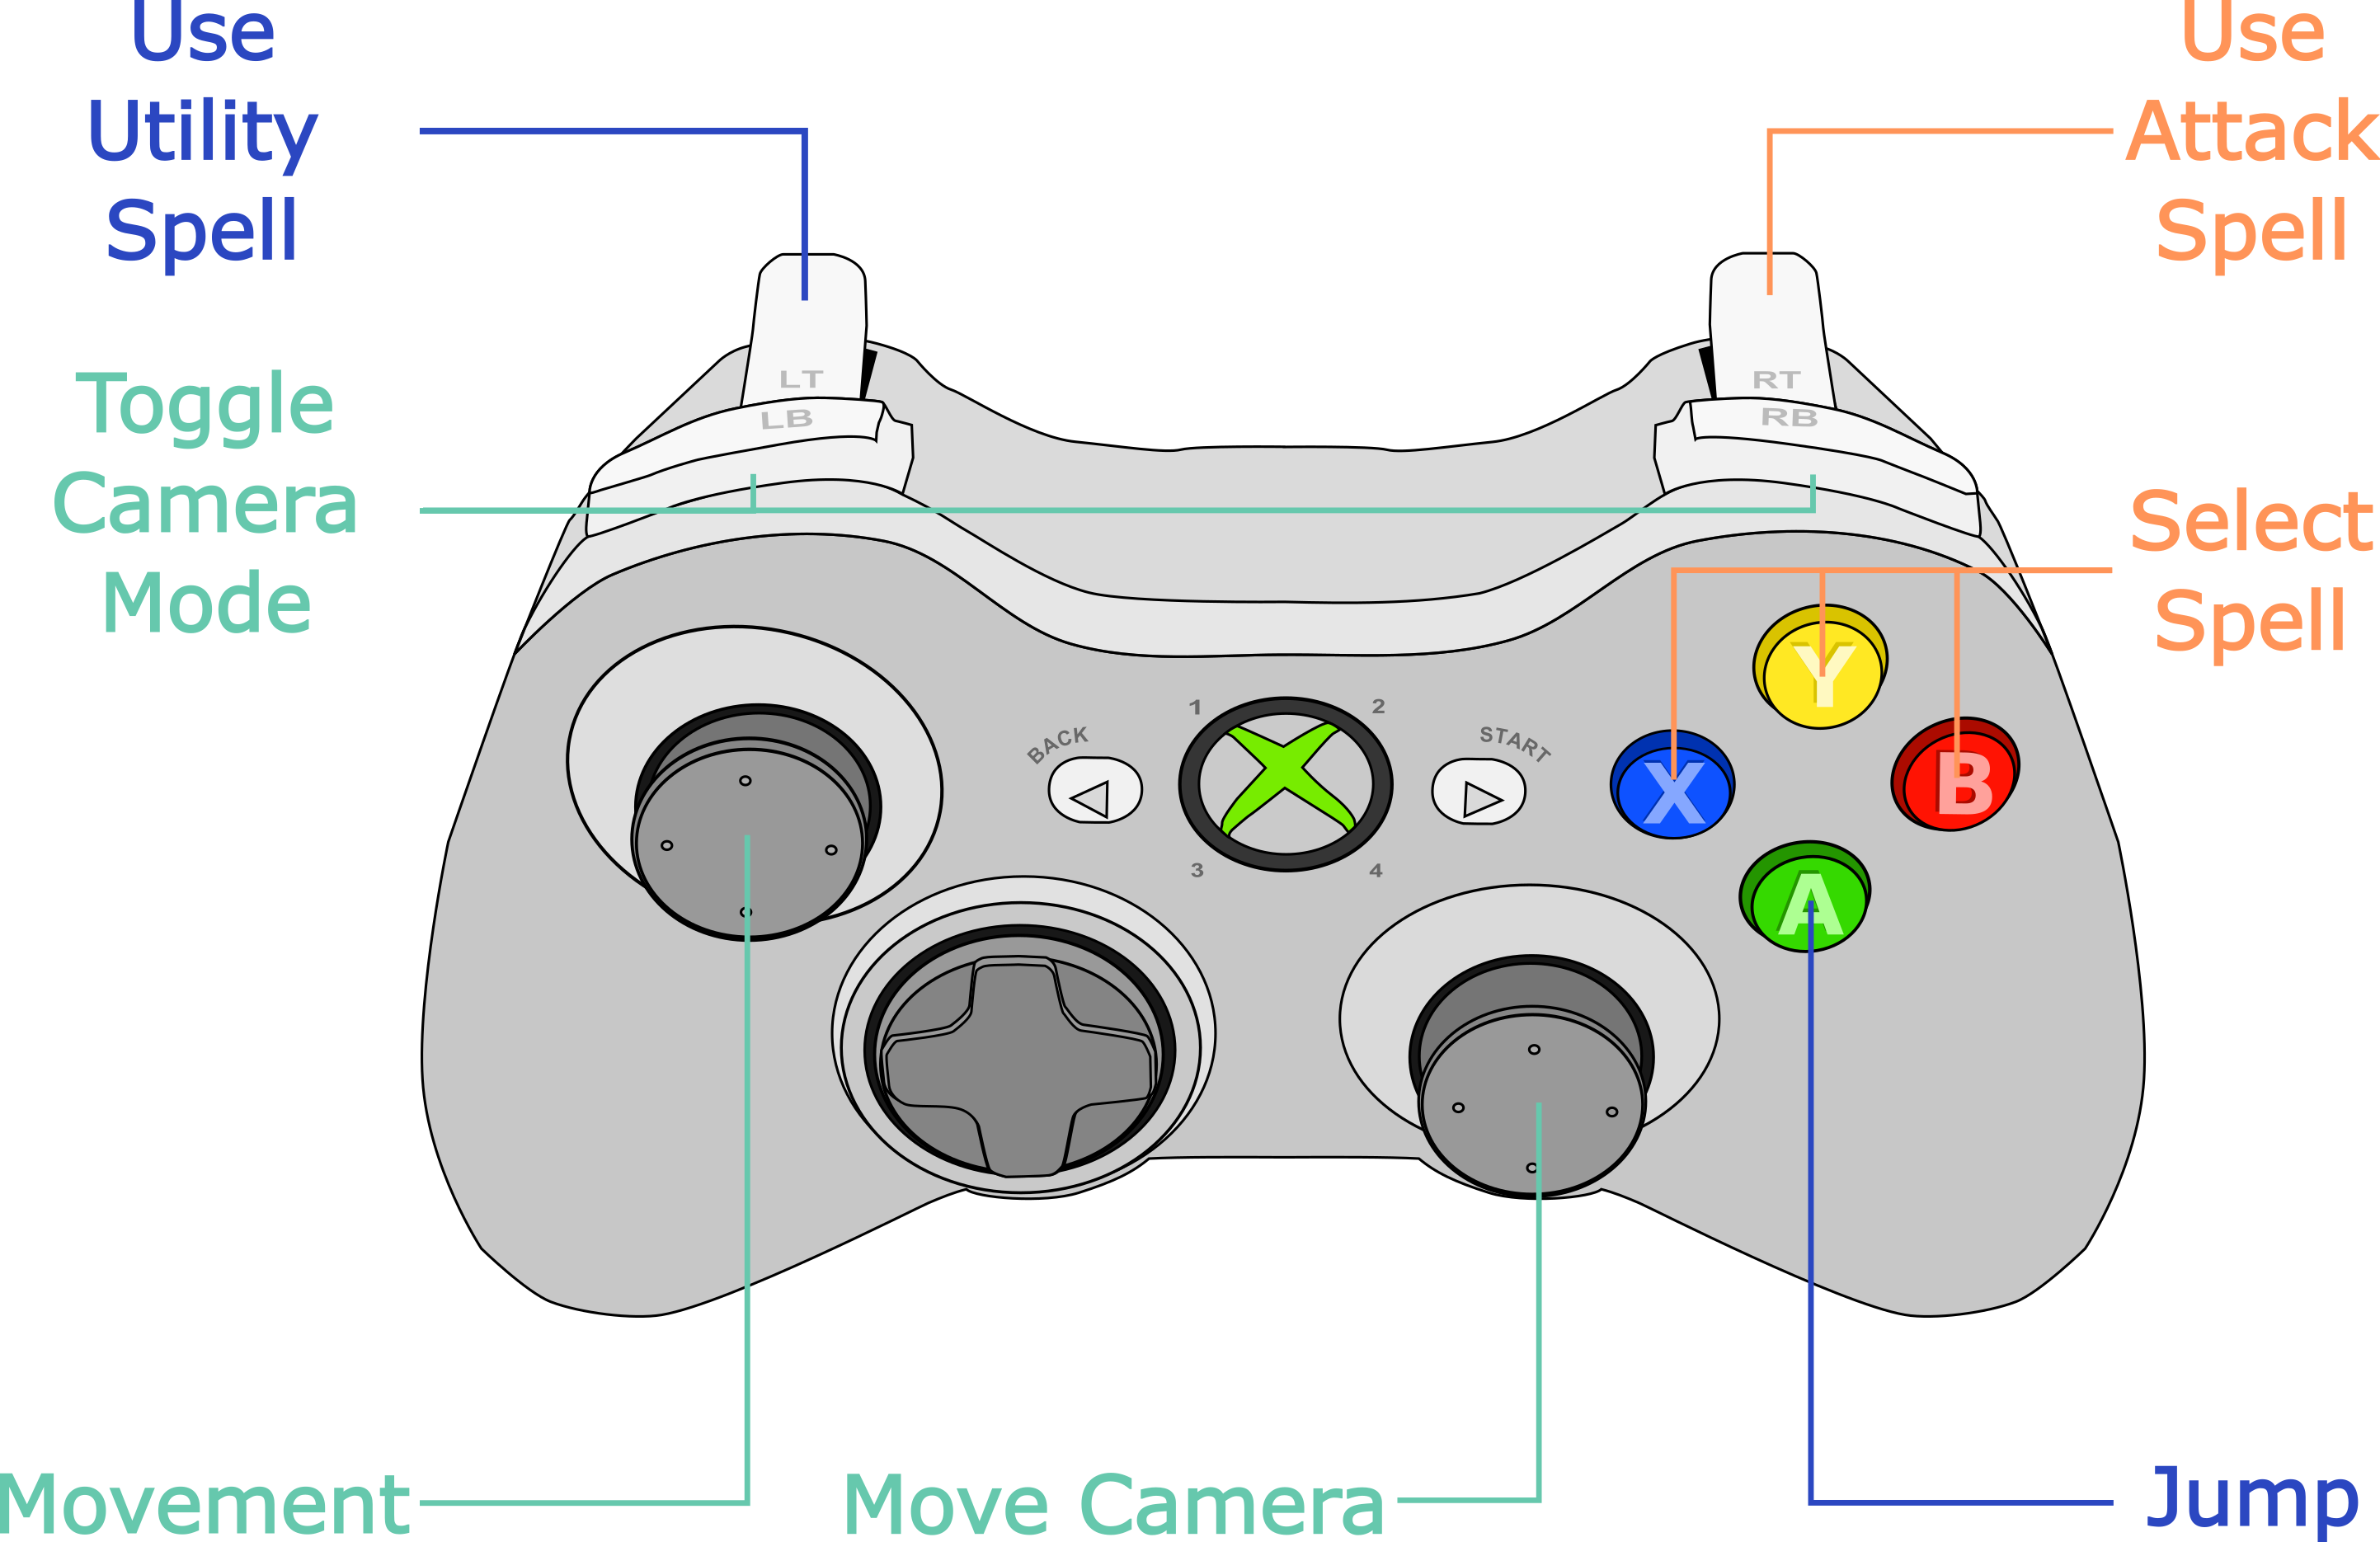
\includegraphics[width=\textwidth]{controller}
    \caption{El control deberá ser completamente configurable, con estos valores por defecto en juego}
\end{figure}

\subsection{Keyboard + Mouse Config}

En caso de no haber controlador XBox o similar disponible puede recurrirse al control mediante teclado y ratón, pero no se recomienda, ya que gran parte del game feel se ha pulido sobre mando y no hay force feedback disponible para este modo de control.

\begin{figure}[h]
    \centering
    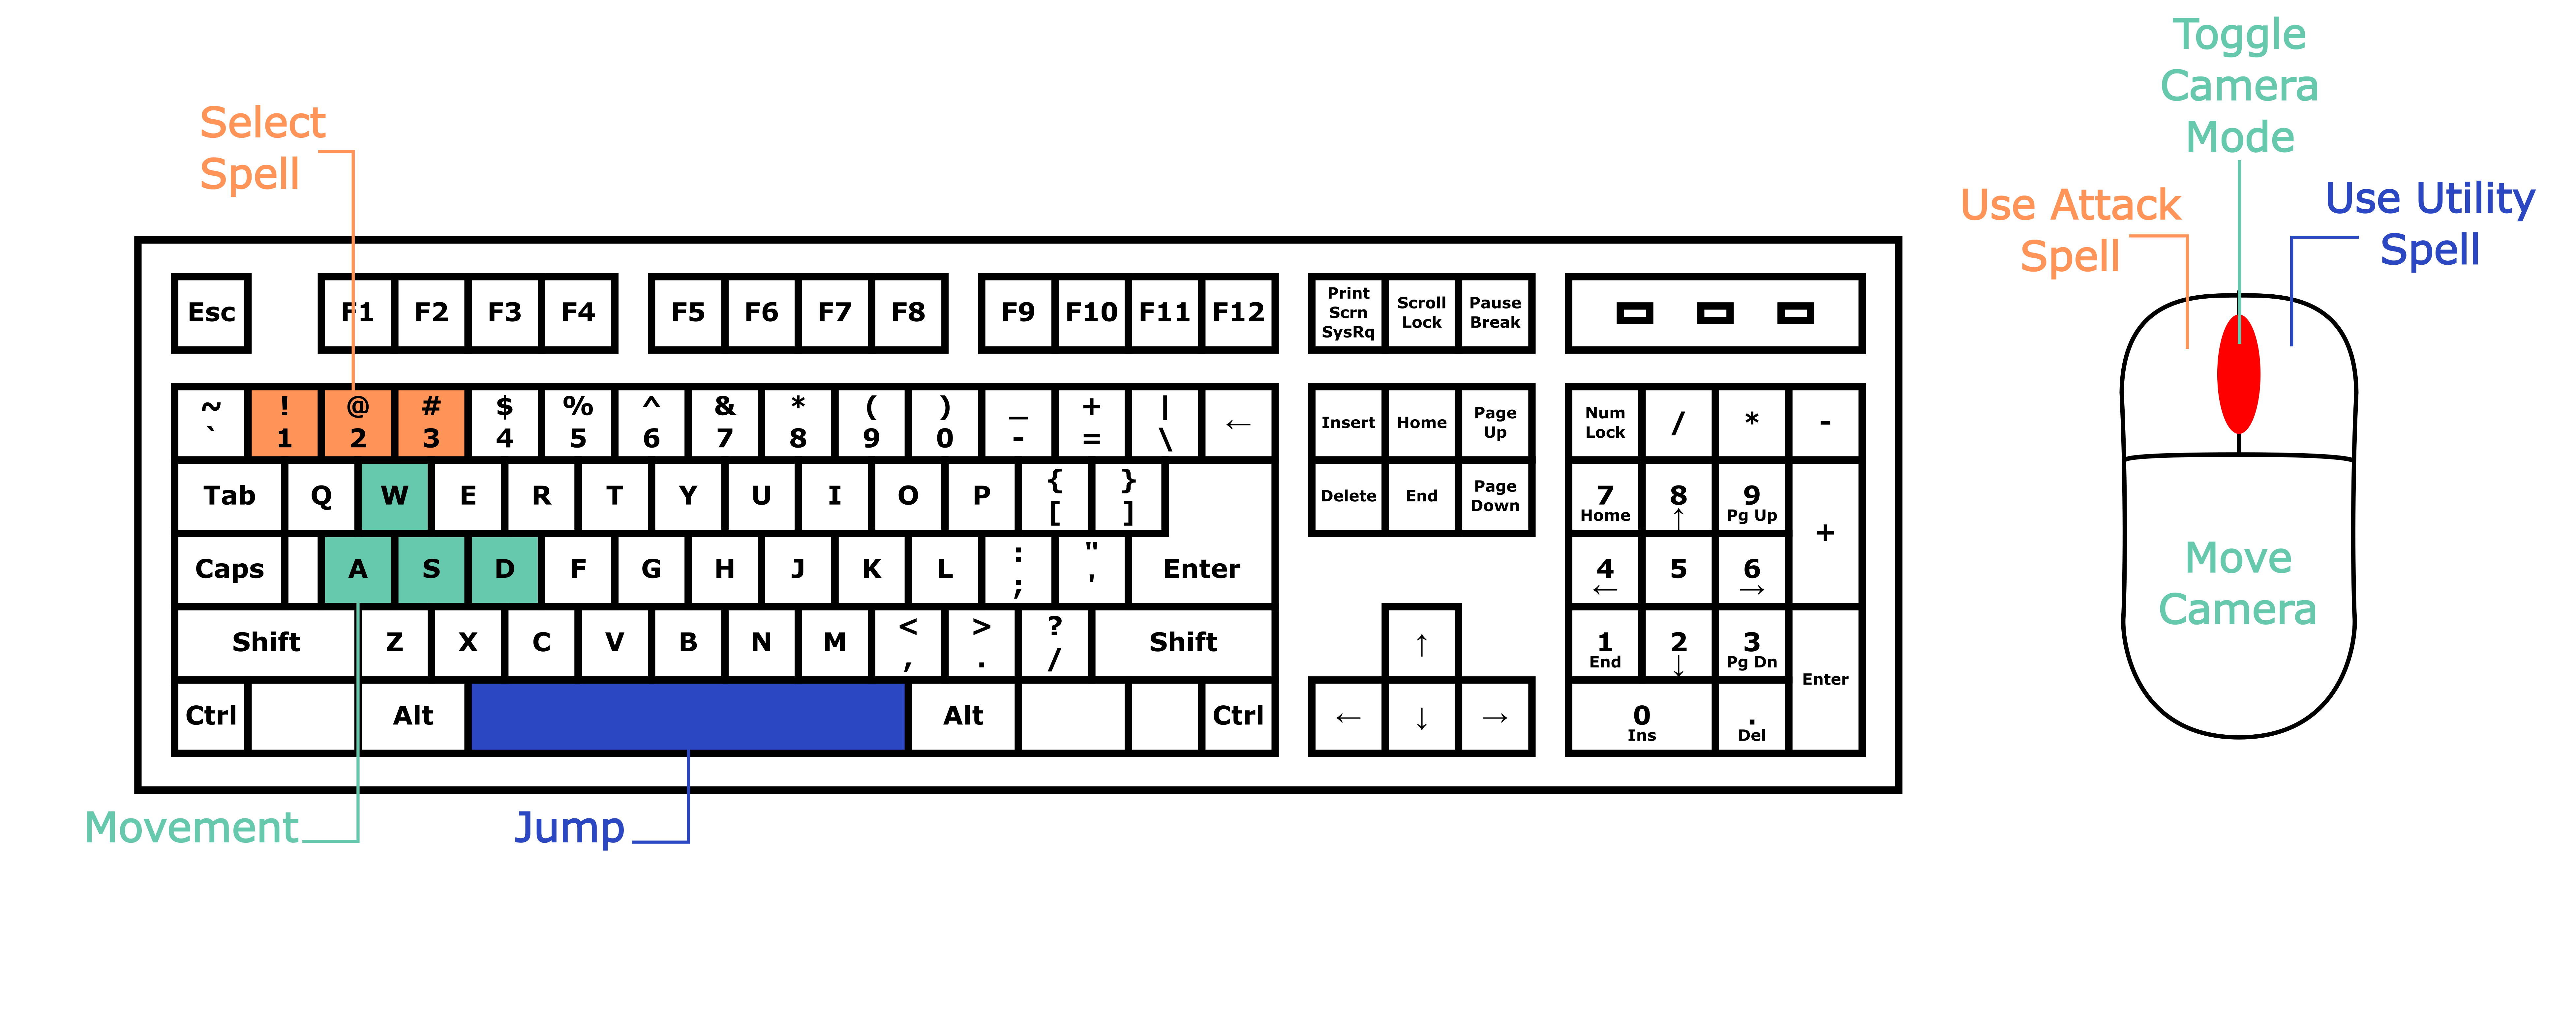
\includegraphics[width=\textwidth]{keyboard}
\end{figure}     

\section{Game Structure}              

\subsection{Tutorial and training}

TBD

Se diseña un nivel de tutorial (ver abajo) en el que el jugador aprenderá los hechizos básicos: la Bola de Fuego, el Escudo Reflector y Cura guiado por un narrador. Una vez el jugador haya superado o rechazado jugar este nivel de tutorial se le permitirá entrar en el modo online y adquirir nuevas habilidades que podrá probar dentro del mismo nivel de tutorial.

\subsection{Accessibility}

Un modo gráfico extra adapta la visibilidad de pantalla para personas con daltonismo.

\subsection{Level Design}

El diseño de los niveles es minimalista y simplificado, para dejar paso a gameplay emergente dadas las habilidades y movimientos de los participantes. Se presenta aquí el diseño básico de un nivel del modo tutorial y otro nivel del modo Capturar la Bandera.

\begin{figure}[H]
    \centering
    
\includegraphics[width=0.8\textwidth]{tutorial}
    \caption{Un nivel de tutorial}
\end{figure}


\begin{figure}[H]
    \centering
    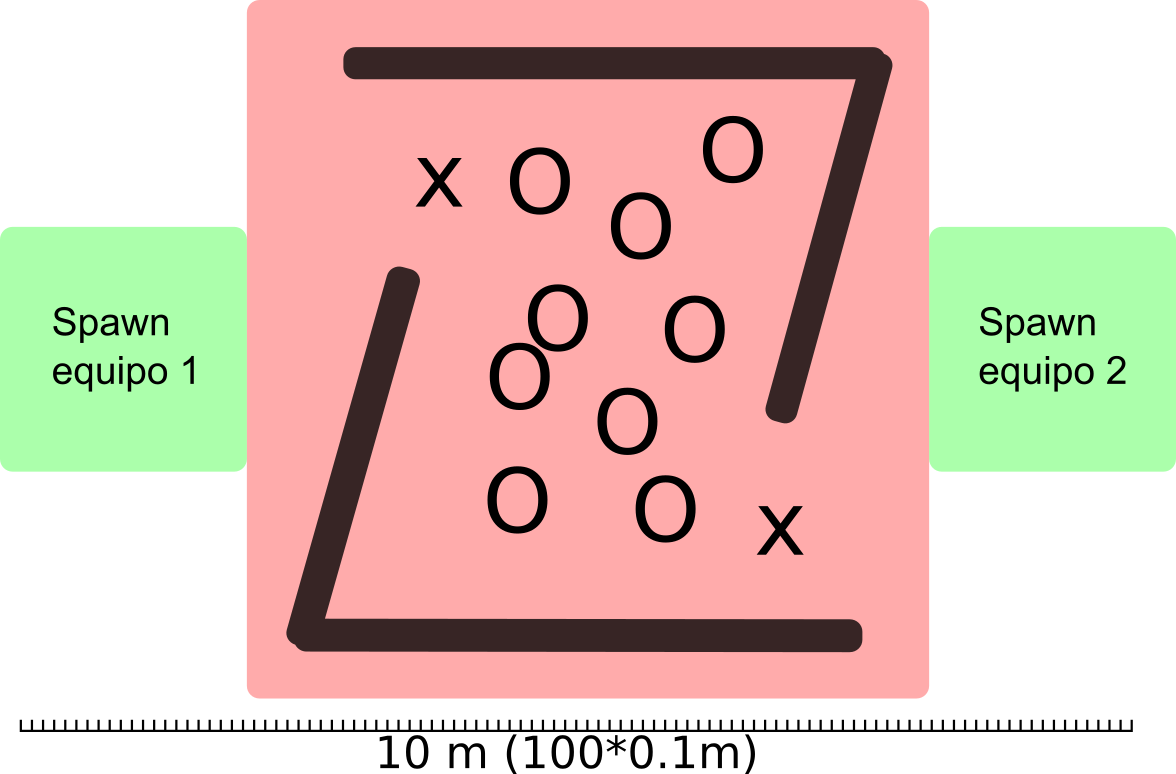
\includegraphics[width=0.7\textwidth]{flags}
    \caption{Un nivel de CTF. Las X representan banderas y los círculos son coberturas destructibles.}
\end{figure}

\part{Technical Details}

\section{Monetization: Game Life Cycle}

La esperanza de vida del juego queda definida como 10.000 jugadores online diarios, ó 7 jugadores concurrentes buscando partida por minuto, ó 1 partida formándose por minuto. Llegado este punto el juego online es claramente insostenible (demasiado tiempo de espera por una partida). Todo plan de negocio planteado para este juego ha de tener este dato en cuenta. Para ello el juego debe ser constantemente rejugable y por tanto han de incluírse quests diarias para reclamar la atención regular del jugador combinado con un gameplay ajustado y dinámico.

Todos los datos de juego (desbloqueos y personalización) se guardan en un sistema de servidores remoto que será accedido por el juego para matchmaking, esto aumenta los costes de mantenimiento del producto. Para costearlos se plantea un flujo de insumos proveniente de la venta de \textit{lootboxes} con contenido estético y nuevos elementos de jugabilidad (hechizos) para los personajes. A largo plazo puede extenderse a nuevos modos de juego o incluso campañas con foco narrativo que extiendan el universo de juego.

\section{Network}

\cleardoublepage

\thispagestyle{empty}

\vspace*{\fill}

\begin{figure}[h]
    \centering
    
\includegraphics[width=0.6\textwidth]{fireball}
\end{figure}

\vfill

\end{document}
